Next we want to show that we have found the general solution to \autoref{eq:diff_eqn_center}.
\begin{lemma}
    The general solution \autoref{eq:diff_eqn_center} is given by $x(t) = a (-\sin t, cos t) + b(\cos t, \sin t)$
\end{lemma}
\begin{proof}
    Suppose $y(t) = (u(t), v(t))$ is another solution to the differential equation. Let $f(t) = (u(t) + iv(t))e^{-it}$. Then
    \begin{align*}
        f'(t) &= (u'(t) + i v'(t)) e^{-it} - ie^{-t} (u(t) + i v(t))\\
        &= (-v(t) + i u(t)) e^{-it} + e^{-it}(-i u(t) + v(t))\\
        &= 0
    \end{align*}
    Therefore $y = \alpha e^{it}$ where $\alpha$ is some complex number implying that $y$ is a linear combination of $X_1(t)$ and $X_2(t)$ as given above.
\end{proof}

\subsubsection{Spiral}
Suppose we have
\begin{equation}\label{eq:spiral}
    X' = \matrix{2 & -1\\1 & 2} X
\end{equation}
We find that the eigenvalues are $\lambda_1 = 2 + i$ and $\lambda_2 = 2 - i$ with corresponding eigenvectors $v_1 = \matrix{i \\ 1}$ and $v_2 = \matrix{-i \\ 1}$. Thus we find that a solution is given by
\begin{align*}
    Z(t) &= e^{(2 + i)t} \left( i \matrix{1\\0} + \matrix{0\\1}\right)\\
    &= e^{2t} (\cos t + i \sin t) \left( i \matrix{1\\0} + \matrix{0\\1}\right)\\
    &= e^{2t} \matrix{-\sin t \\ \cos t} + i e^{2t} \matrix{\cos t \\ \sin t}
\end{align*}
Thus the two solutions are given by the real and the imaginary parts:
$$ X_1(t) = e^{2t} \matrix{-\sin t \\ \cos t}, X_2 =  e^{2t} \matrix{\cos t \\ \sin t}$$
The general solution is then of course some linear combination of $X_1$ and $X_2$.

Consider $X_1(t)$. As $t$ increases the $(-\sin t, \cos t)$ component makes the point go around in the origin (with period $2\pi$) while the $e^{2t}$ causes the magnitude to increase. Thus we get a spiraling out. In order to determine the direction of the spiral (i.e. clockwise or counterclockwise) we can either investigate $(-\sin t, \cos t)$ (as $t$ increases the $x-$coordinate decreases while the $y-$coordinate increases, therefore counterclockwise) or we can try a point and determine which way the the tangent vector points. For example substituting $X = (1, 0)$ into \autoref{eq:spiral} we find that $X' = (2, 1)$ implying that that the spiral must be going counterclockwise.


\begin{figure}[h]
    \centering
    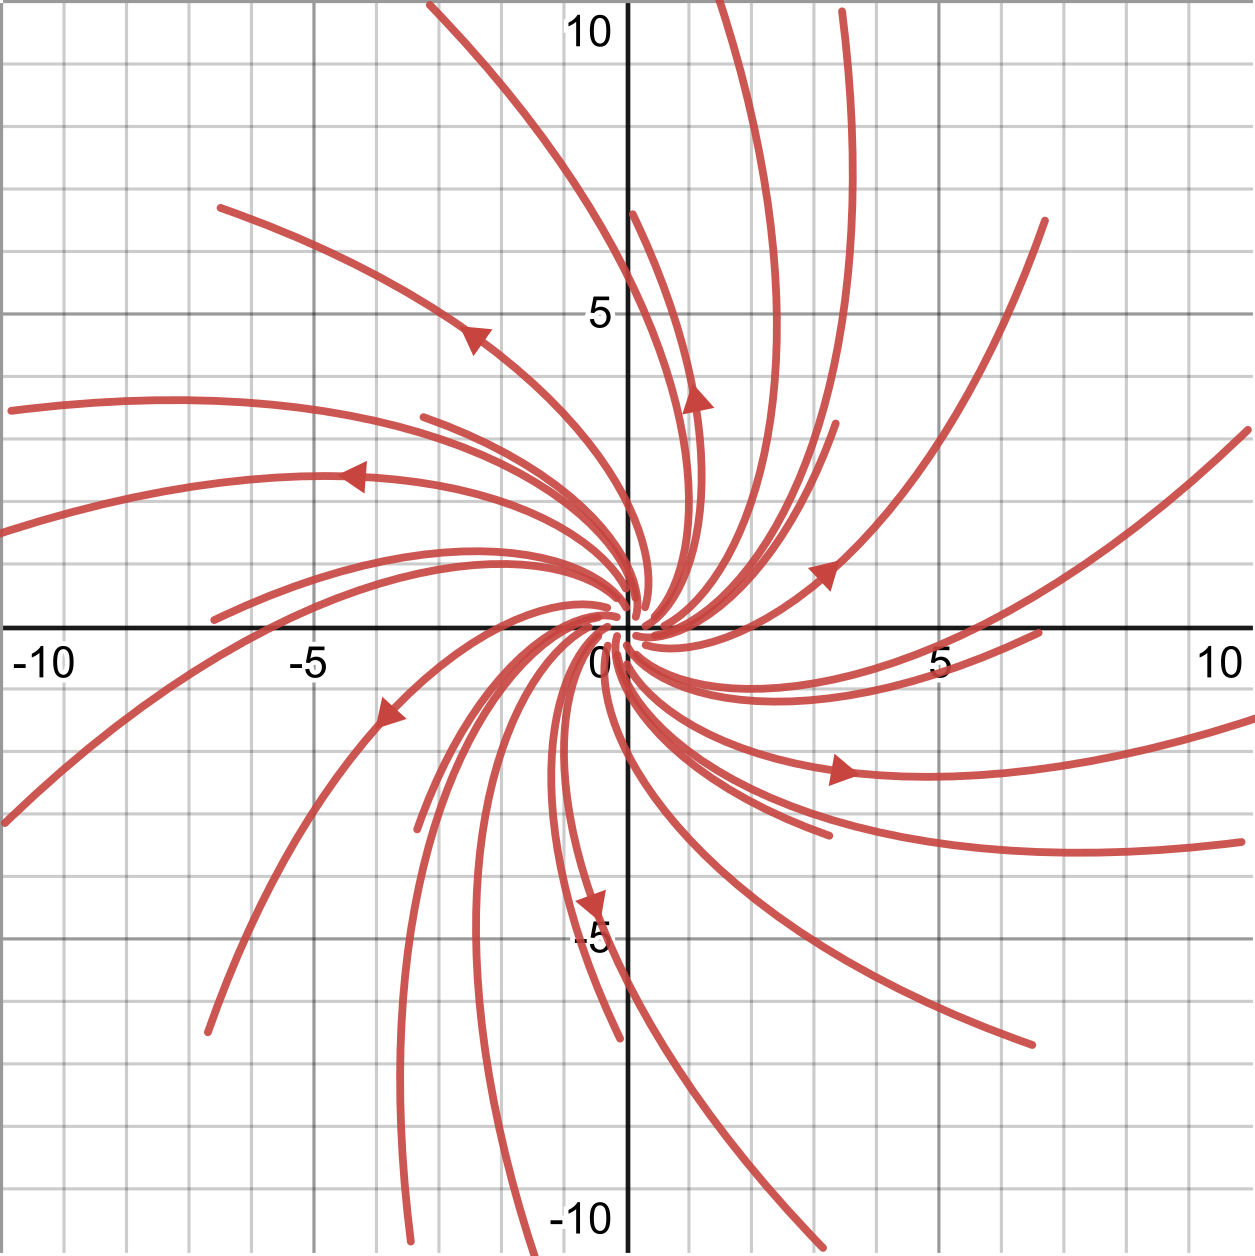
\includegraphics[scale=0.25]{Images/spiral.png}
    \caption{Spiral (counterclockwise)}
    \label{fig:sprial-cc}
\end{figure}

\subsection{Repeated eigenvalues (Part I)}
Suppose we have
\begin{equation}
    X' = \matrix{3 & -1\\4 & -1} X
\end{equation}
where we will denote matrix by $A$, as usual. The characteristic polynomial of $A$ is $\lambda^2 - 2\lambda + 1$ which has a repeated root for $\lambda = 1$. Hence 1 is an eigenvalue with algebraic multiplicity 2. However $A - I$ is a matrix of rank 1, hence there is only one eigenvector namely $v = \matrix{1\\2}$. This is gives one solution with
$$ X_1(t) = c e^{t} \matrix{1\\2} $$
However we expect a two dimensional solution space (a statement which we will justify later) hence we know there should be one other linearly independent solution.

From the study of linear algebra, we recall in this case $A$ must have a basis in generalised eigenvectors. In this we can compute the generalised eigenvector of $A$ is $w = \matrix{0\\-1}$. Hence we might expect the second solution to be of the form $X(t) = \alpha(t) v + \beta(t)w$ with $\beta \neq 0$ (the case with $\beta = 0$ is covered by $X_1$ above). Assuming that $X(t)$ does solve our differential equation we see that
\begin{align*}
    X'(t) &= A(\alpha(t)v + \beta(t)w)\\
    &= \alpha(t)Av + \beta(t)Aw\\
    &= \alpha(t)\lambda v + \beta(t)(\lambda w + v)\\
    &= (\lambda \alpha(t) + \beta(t))v + \lambda \beta(t) w
\end{align*}
On other hand we also know that
$$ X'(t) = \alpha'(t) v + \beta'(t) w $$
equating coefficients (since $(v, w)$ is a basis, the coefficients are unique), we get the following system of equations
\begin{align*}
    \begin{cases}
    \alpha' = \lambda \alpha + \beta\\
    \beta' = \lambda \beta
    \end{cases}
\end{align*}
The second equation is easily solved by $\beta(t) = c e^{\lambda t}$ where $c$ can be any constant (in fact, as we know, the equation is \textit{only} solved by this). Recall that we are trying find a \textit{particular} solution to the differential equation (one that is linearly independent of $X_1$). Hence, for simplicity, we can take $c = 1$ above giving us $\beta(t) = e^{\lambda t}$.

This, however, leaves us to solve to solve for $\alpha$. One might expect that we can simply use the theory built up so far since this is simply a homogeneous, linear system of equations. However, one can check that this system is exactly the case we are considering right now: the case with repeated eigenvalues with a basis in generalised eigenvectors. Therefore we will have to resort to some combination of guesswork and being clever. 

In this case, we recall that the homogeneous equation $\alpha' = \lambda \alpha$ would be solved by $\alpha(t) = c e^{\lambda t}$ where $c$ is a constant. One might guess that if instead we vary the constant in some appropriate manner (i.e. make it a function of $t$), we might be able to solve for $\alpha'(t) = \lambda \alpha(t) + e^{\lambda t}$. Therefore suppose $\alpha(t) = y(t) e^{\lambda t}$. Assuming this to be a solution, we get
\begin{align*}
    \alpha'(t) = y'(t) e^{\lambda t} + \lambda y(t) e^{\lambda t}
\end{align*}
It is then clear that if $y'(t) = 1$ then we have a solution. In other words we can take $y(t) = ct$ for any constant $c$. Once again we are only interested in one particular solution. Therefore, we take the simplest one to conclude that $\alpha(t) = te^{\lambda t}$. We then finally have a second, linearly independent solution to our ODE:
$$ X_2(t) = te^{\lambda t} v + e^{\lambda t}w $$
In other words the general solution to the ODE is given by
\begin{align*}
    X(t) = a_1 X_1(t) + a_2 X_2(t)
\end{align*}
where $a_1, a_2$ are constants determined by the initial conditions, as usual.

Let us substitute the specific values of $\lambda, v$ and $w$ to get a clearer picture of the solutions (everything thus far will hold for any repeated eigenvalues with a basis in generalised eigenvectors). We have that our solution is given by
\begin{align*}
    X(t) &= a_1 e^{t} \matrix{1\\2} + a_2 \left( t e^{t} \matrix{1\\2} + e^{t} \matrix{0\\-1} \right)\\
    &= a_1 e^{t} \matrix{1\\2} + a_2 e^{t} \left( t \matrix{1\\2} + \matrix{0\\-1}  \right)\\
    &= (a_1 e^{t} + a_2 t e^{t}) \matrix{1\\2} + a_2 e^{t} \matrix{0\\-1}
\end{align*}

We see that as $t \to \infty$ the component corresponding to $\matrix{1\\2}$ increases much more quickly that its partner, implying that the solution curves become increasing parallel to the line spanned by $\matrix{1\\2}$. On the other hand as $t \to -\infty$, this component also approaches 0 more quickly, so in the limit the solution curves becomes tangent to $\matrix{1\\2}$ at the origin. If the eigenvalue were negative, then things remain essentially identical except the arrows are reversed.

% TODO: Add diagram for repeated eigenvalues, positive and negative

\subsection{Repeated Eigenvalues (Part II)}
It's possible that one has repeated eigenvalues \textit{and} a basis of eigenvectors. An example is
\begin{equation}
    X' = \matrix{2 & 0 \\ 0 & 2} X
\end{equation}
where the standard basis vectors are eigenvectors themselves. In this case every vector is an eigenvector. Although the example might seem like a special case, it in fact highlights the general case since the assumptions on the matrix mean that it is a multiple of the identity. If it's a positive multiple of the identity (like the example above), then everything tends away from the origin in the direction parallel to itself. Note how extremely unstable this is since the mildest of perturbations cases the long term behaviour to be completely different. If we have a negative multiple of the identity, then the situation reverses and everything approaches the origin (and of course this is a very stable situation: regardless of where you start, you tend towards the origin).

% TODO: Add diagram for repeated eigenvalues, basis of eigenvectors, positive and negative

\section{Trace-Determinant Plane}
% TODO: Add trace-determinant plane diagram
We are interested in classifying the different dynamical systems, roughly based on what the phase portraits look like. For example, all centers are roughly the same (the only thing that varies is the frequency and the direction of the rotation); all saddle points are essentially the same (up to some rotation and stretching), etc. What we realise is that almost all of this information is determined by the eigenvalues and in particular by the sign of the eigenvalues, whether they are real or complex, etc. If we can then work out the relationships between the eigenvalues (ideally without solving for them), we can classify the dynamical systems relatively easily.

This is where we remember from our study of linear algebra that the eigenvalues of a matrix can by found by looking at the roots of the characteristic polynomial of the matrix and in the $2 \times 2$ case, this polynomial is completely determined by the trace and determinant. Indeed we have that the characteristic polynomial $p_A$ of a $2 \times 2$ matrix $A$ is given by
$$ p_A(\lambda) = \lambda^2 - \Tr(A)\lambda + \det(A) $$
We know then, for example, that if the discriminant of the above quadratic is positive, then we have 2 distinct real eigenvalues. If in addition the determinant is positive, then we know the eigenvalues share sign. Finally we can use the trace to determine what exactly their sign is. This gives us a near complete description of the qualitative behaviour of $A$. Repeating this analysis for the other cases, we summarise our findings below.

\renewcommand{\arraystretch}{1.2}
\begin{table}[h]
    \centering
    \begin{tabular}{c|c|c|c}
    Eigenvalues & Normal form & How to detect & Shape\\
    \hline
    $\lambda_1 > \lambda_2 > 0$ & $\matrix{\lambda_1 & 0\\0 & \lambda_2}$ & $\Tr(A)^2 > 4 \det(A)$ & Unstable node  \\
    $\lambda_1 > 0 > \lambda_2$ & $\matrix{\lambda_1 & 0\\0 & \lambda_2}$ & $\det(A) < 0$ & Saddle\\
    $0 > \lambda_1 > \lambda_2$ & $\matrix{\lambda_1 & 0\\0 & \lambda_2}$ & $\det(A) > 0$, $\Tr(A) < 0$ & Stable node\\
    $\lambda = \alpha + i\beta$, $\alpha > 0$ & $\matrix{\alpha & -\beta \\ \beta & \alpha}$ & $\Tr(A) > 0, 4\det(A) > \Tr(A)^2$ & Spiral source\\
    $\lambda = \alpha + i\beta, \alpha < 0$ & $\matrix{\alpha & -\beta \\ \beta & \alpha}$ & \makecell{$\det(A) > 0, \Tr(A) < 0$ \\ $4\det(A) < \Tr(A)^2$} & Spiral sink
    \end{tabular}
    \caption{Generic cases for $X' = AX$}
    \label{tab:gen-cases}
\end{table}

These are the generic cases (to defined more precisely later), but roughly speaking, this is what `most' $2 \times 2$ matrices look like: they either have 2 distinct eigenvalues or 2 complex eigenvalues (which are conjugates). This can be verified by the fact that the above cases have covered almost all of the trace-determinant plane.

There do remain, however, some degenerate or exceptional cases that we still need to verify. In general these occur when we have an equality of some kind (in other words something is equal to 0 and as one can imagine this is rarely a good thing). These are summarised in \autoref{tab:degen-cases}.

\begin{table}[h]
    \centering
    \begin{tabular}{c|c|c|c}
    Eigenvalues & Normal form & How to detect & Shape\\
    \hline
    $\lambda = i \beta$ & $\matrix{0 & -\beta\\ \beta & 0}$ & $\Tr(A) = 0, \det(A) > 0$ & Center\\
    $\lambda_1 = \lambda_2 > 0$ & $\matrix{\lambda_1 & 1\\ 0 & \lambda_1}$ & \makecell{$\Tr(A)^2 = 4\det(A)$, \\rank$(A - \lambda_1 I) = 1, \Tr(A) > 0$} & Unstable, source\\
    $\lambda_1 = \lambda_2 < 0$ & $\matrix{\lambda_1 & 1\\ 0 & \lambda_1}$ & \makecell{$\Tr(A)^2 = 4\det(A)$, \\rank$(A - \lambda_1 I) = 1, \Tr(A) < 0$} & Stable, sink\\
    $\lambda_1 = \lambda_2 > 0$ & $\matrix{\lambda_1 & 0\\ 0 & \lambda_1}$ & $A = \lambda_1 I, \Tr(A) > 0$ & (Very) unstable, source\\
    $\lambda_1 = \lambda_2 < 0 $ & $\matrix{\lambda_1 & 0\\ 0 & \lambda_1}$ & $A = \lambda_1 I, \Tr(A) < 0$ & Stable, sink\\
    $\lambda_1 > 0, \lambda_2 = 0$ & $\matrix{\lambda_1 & 0\\0 & 0}$ & $\det(A) = 0, \Tr(A) > 0$ & Unstable\\
    $\lambda_1 < 0, \lambda_2 = 0$ & $\matrix{\lambda_1 & 0\\0 & 0}$ & $\det(A) = 0, \Tr(A) < 0$ & Stable\\
    $\lambda_1 = \lambda_2 = 0$ & $\matrix{0 & 1\\0 & 0}$ & $\Tr(A) = \det(A) = 0,$ rank$(A) = 1$ & Unstable\\
    $\lambda_1 = \lambda_2 = 0$ & $\matrix{0 & 0\\0 & 0}$ & $A = 0$ & Constant
    \end{tabular}
    \caption{Degenerate cases for $X' = AX$}
    \label{tab:degen-cases}
\end{table}
We say a bifurcation occurs in an ODE when change the parameters a bit causes the qualitative behaviour to change drastically (for example changing from a source to a sink). This is a definition we will make more precise later. These information is often summarised in a bifurcation diagram. Note that the trace-determinant plane is an example of a bifurcation diagram where the axes and curves are used to group similarly behaved equations together and bifurcations occur when we go from one region to another.


